\section{Durchführung}
\label{sec:Durchführung}

Zum weiter Vorgehen muss zurnächst die Federstärke $D$ der Feder bestimmt werden.
Dafür wird an der Drehachse an der die Feder befestigt ist, ein Stab senkrecht zur Drehachse eingespannt.
Dieser wird nun jeweils um 30 Grad gedreht, daraufhin wird mit einem Newtonmeter die Kraft gemessen, welche die Feder in einem gewissen Abstand ausübt.
Nach zehn Messungen von 30 Grad bis 300 Grad, werden an dem Stab zwei Gewichte angebracht.
Die Masse und Ausdehung der Gewichte wurde zuvor durch Messungen bestimmt.
Die Massen werden als erstes ganz außen auf dem Stab in einem Abstand von $\SI{28.5}{\centi\meter}$ angebracht.
Der Aufbau ist in Abbildung \ref{fig:StabmitGewicht} zu sehen
Nun wird der Stab gedreht und die Feder damit Ausgelenkt.
Daraufhin wird der Stab losgelassen und die Schwingungsdauer $T$ einer Periode gemessen und notiert.
Dieser Prozess wird mit verschieden Abständen zur Drehachse wiederholt.
Nachdem zehn Werte aufgenommen wurden wird der Aufbau erneut umgebaut.

\begin{figure}
\centering
\caption{Versuchsaufbau mit zwei Gewichten an einem langem Stab.}
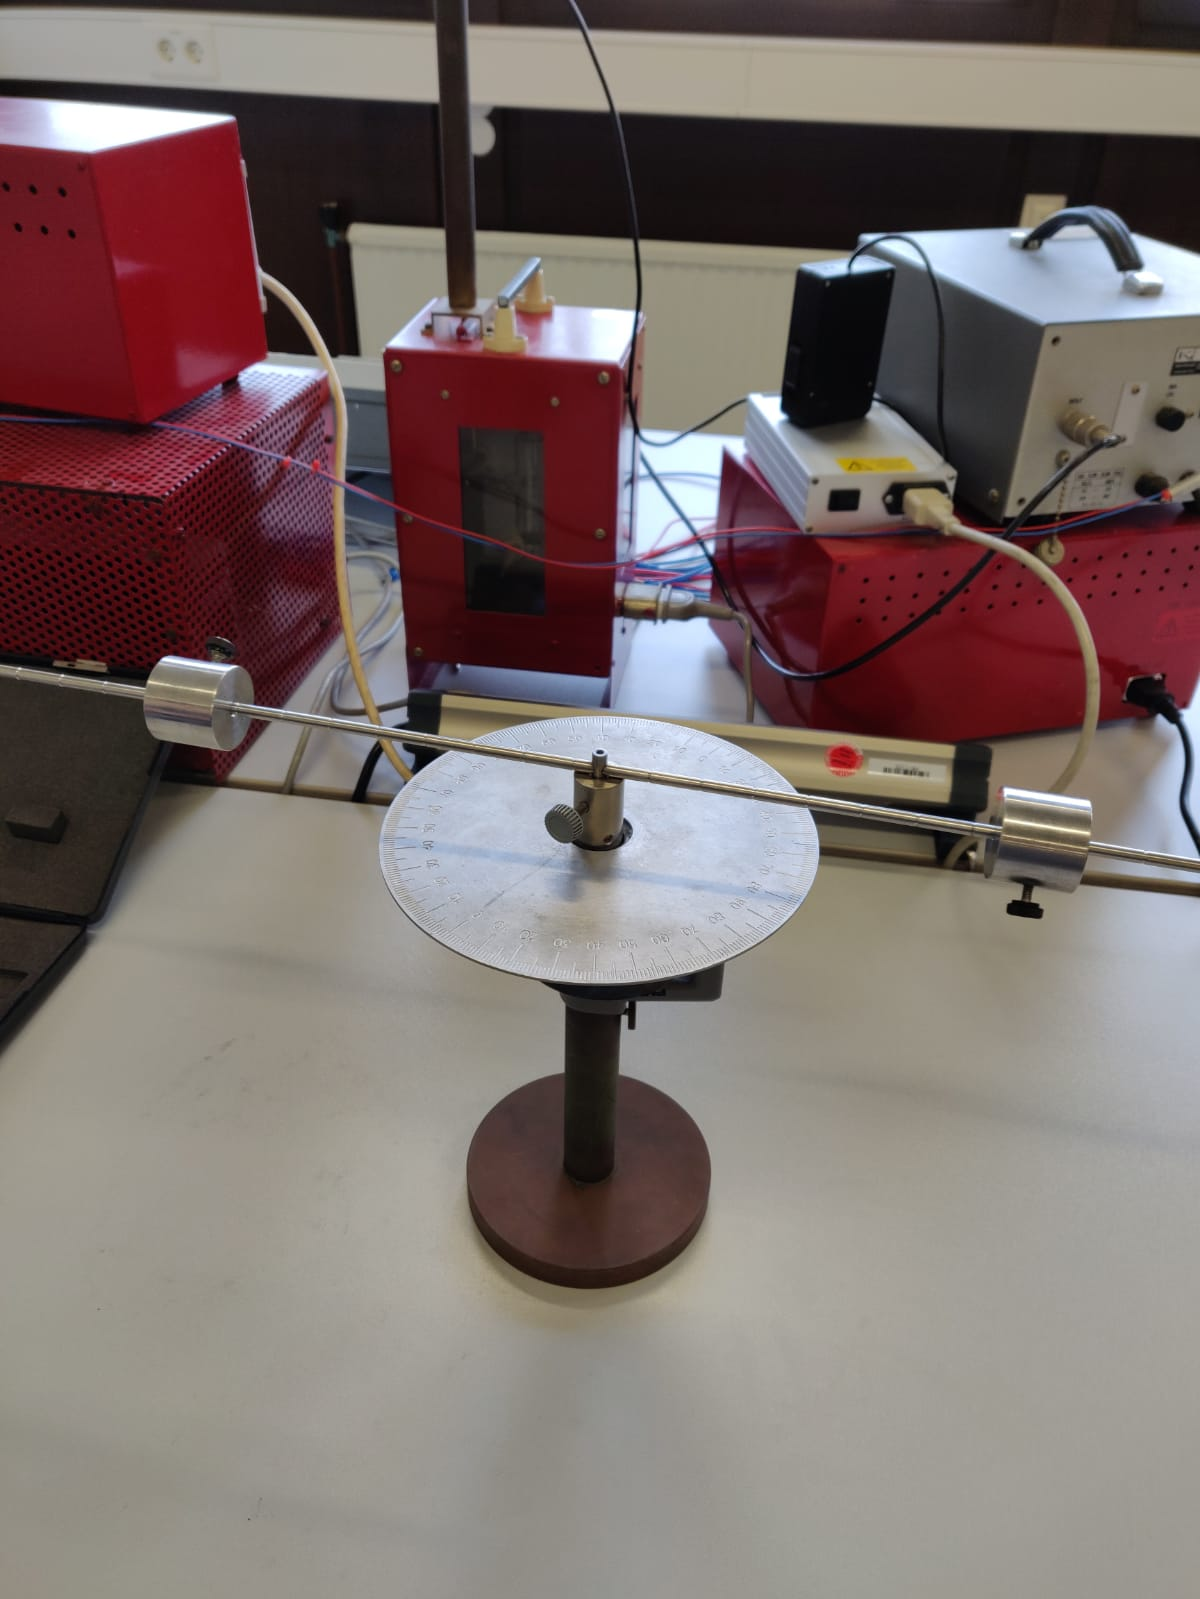
\includegraphics[scale=0.1]{content/data/StabmitGewichten.png}
\label{fig:StabmitGewicht}
\end{figure}

\subsection{Trägheitsmomente von Körpern}
\FloatBarrier
Nun werden verschiedene Körper auf der Drehachse angebracht.
Zuerst wird ein großer Zylinder auf der Drechachse eingespannt.
Die Ausdehnung und Masse des Zylinders wurden vorher bestimmt.
Dieser wird um einen Winkel ausgelenkt und wieder losgelassen.
Nach dem Loslassen wird die Schwingungsdauer gemessen und notiert.
Um einen möglichst genauen Mittelwert zu bekommen wird der Prozess fünf mal mit gleichen Auslenkungen durchgeführt.

Daraufhin wird der große Zylinder mit einem anderen Körper getauscht.
Der nächste körper ist ein kleiner liegender Zylinder.
Der Aufbau ist in der Abbildung \ref{fig:ZylinderStehend} zu sehen.
Auch die Ausdehung und Masse dieses Körpers wurden vorher bestimmt.
Dieser wird nun genau wie der große Zylinder auf der Drehachse eingespannt und um einen bestimmten Winkel ausgelenkt.
Auch hier wird die Schwingungsdauer fünf mal gemessen um den Mittelwert möglichst genau zu bestimmen.
\FloatBarrier
\begin{figure}
\centering
\caption{Versuchsaufbau mit einem stehenden Zylinder}
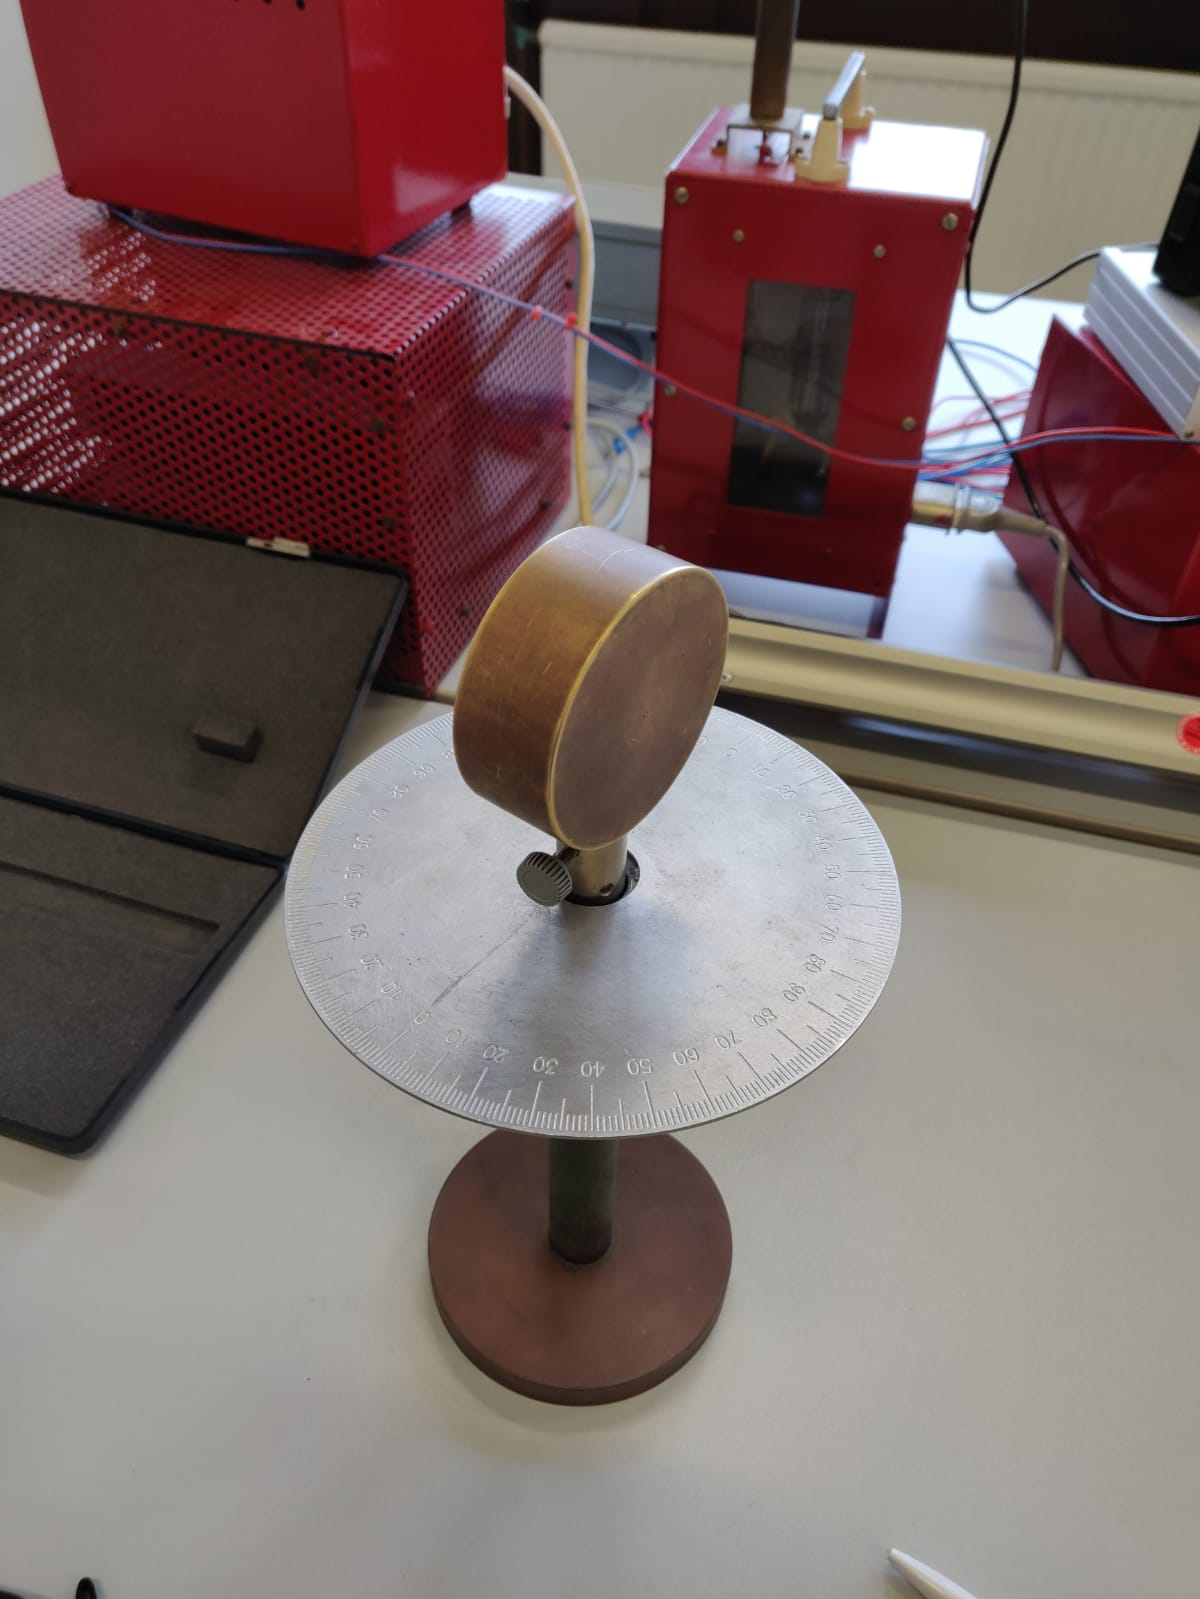
\includegraphics[scale=0.1]{content/data/ZylinderStehend.png}
\label{fig:ZylinderStehend}
\end{figure}

\FloatBarrier
Nun wird anstelle des Zylinders eine Puppe auf der Drehachse montiert, diese ist in Abbildung \ref{fig:puppesitzend} zu sehen.
Auch diese wird bis zu einem gewissen Winkel ausgelenkt und losgelassen.
Daraufhin wird wieder die Schwingungsdauer notiert.
Auch dieser Prozess wird fünf mal wiederholt.
Daraufhin wird die Puppe in eine andere Position gebracht, diese ist in Abbildung \ref{fig:puppetpose} zu sehen.
Hier wird wie bei der anderen Puppen Position vorgegangen.

\begin{figure}
\centering
\begin{subfigure}{0.5\textwidth}
    \centering
    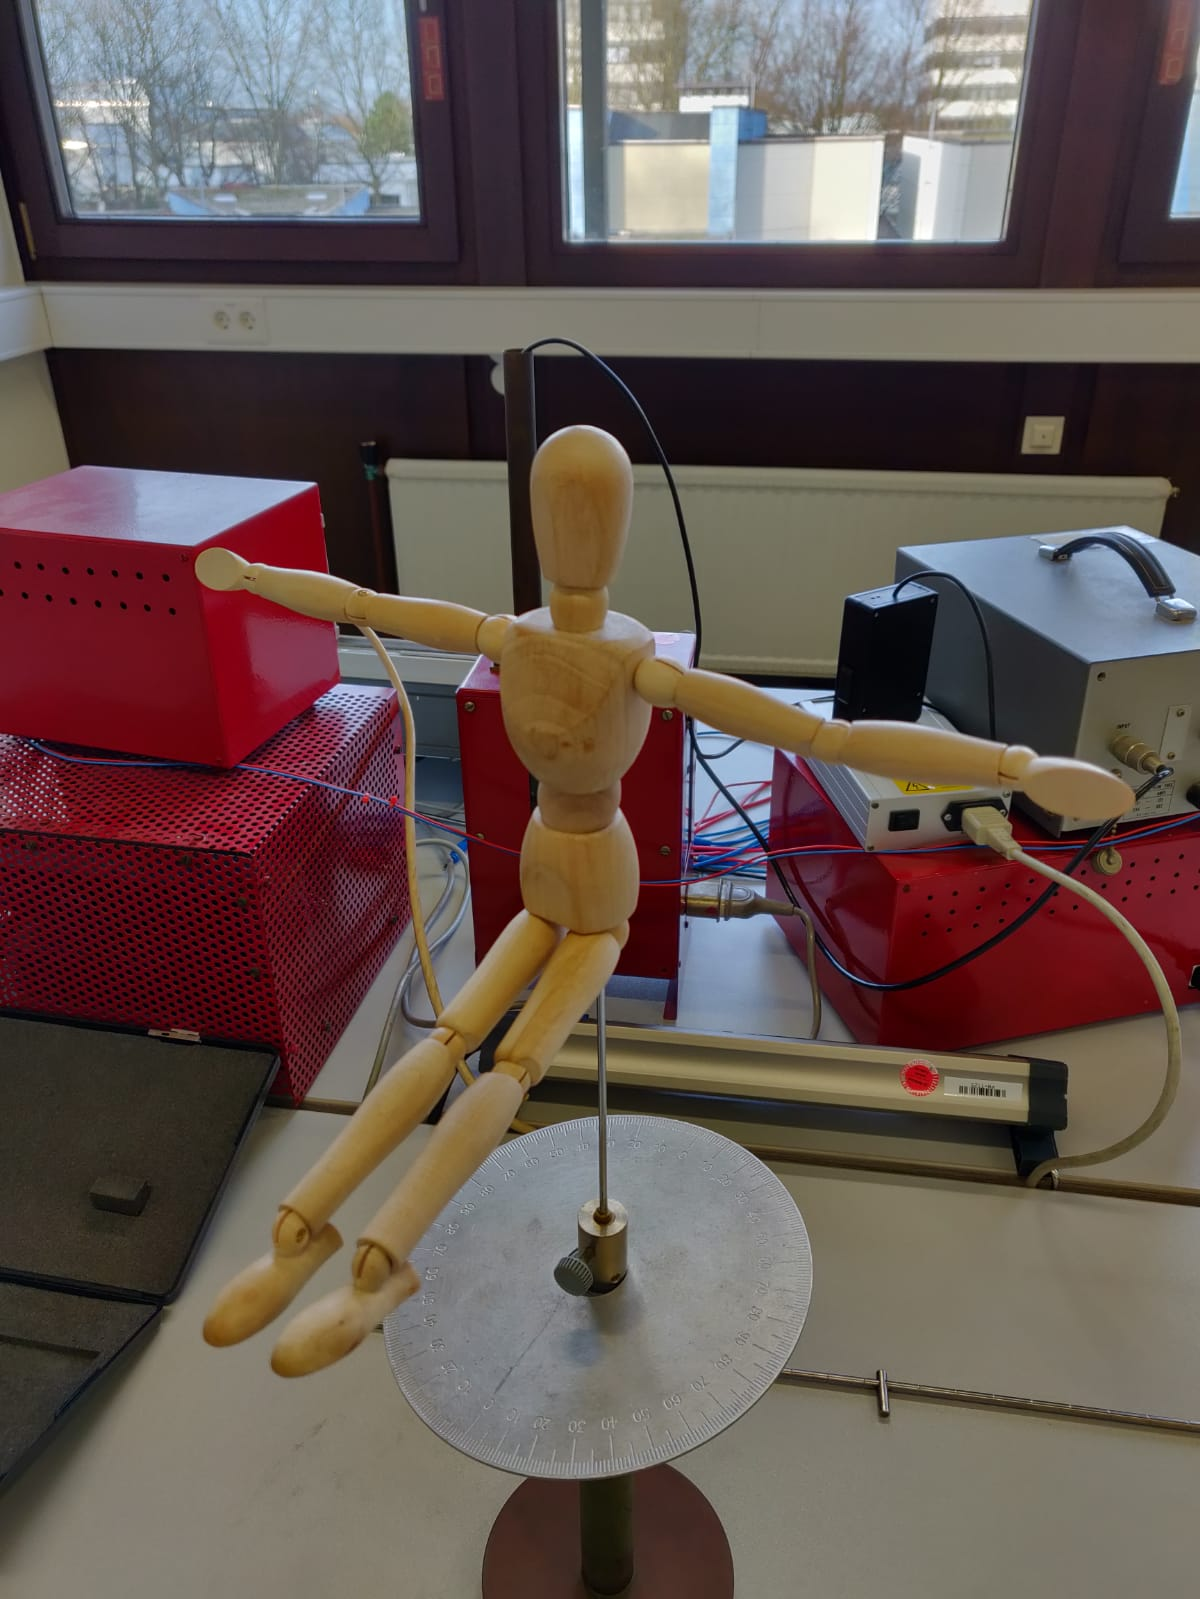
\includegraphics[scale=0.1]{content/data/PuppeSitzend.png}
    \caption{Versuchsaufbau mit einer stehenden Puppe.}
    \label{fig:puppesitzend}
\end{subfigure}%
\begin{subfigure}{0.5\textwidth}
    \centering
    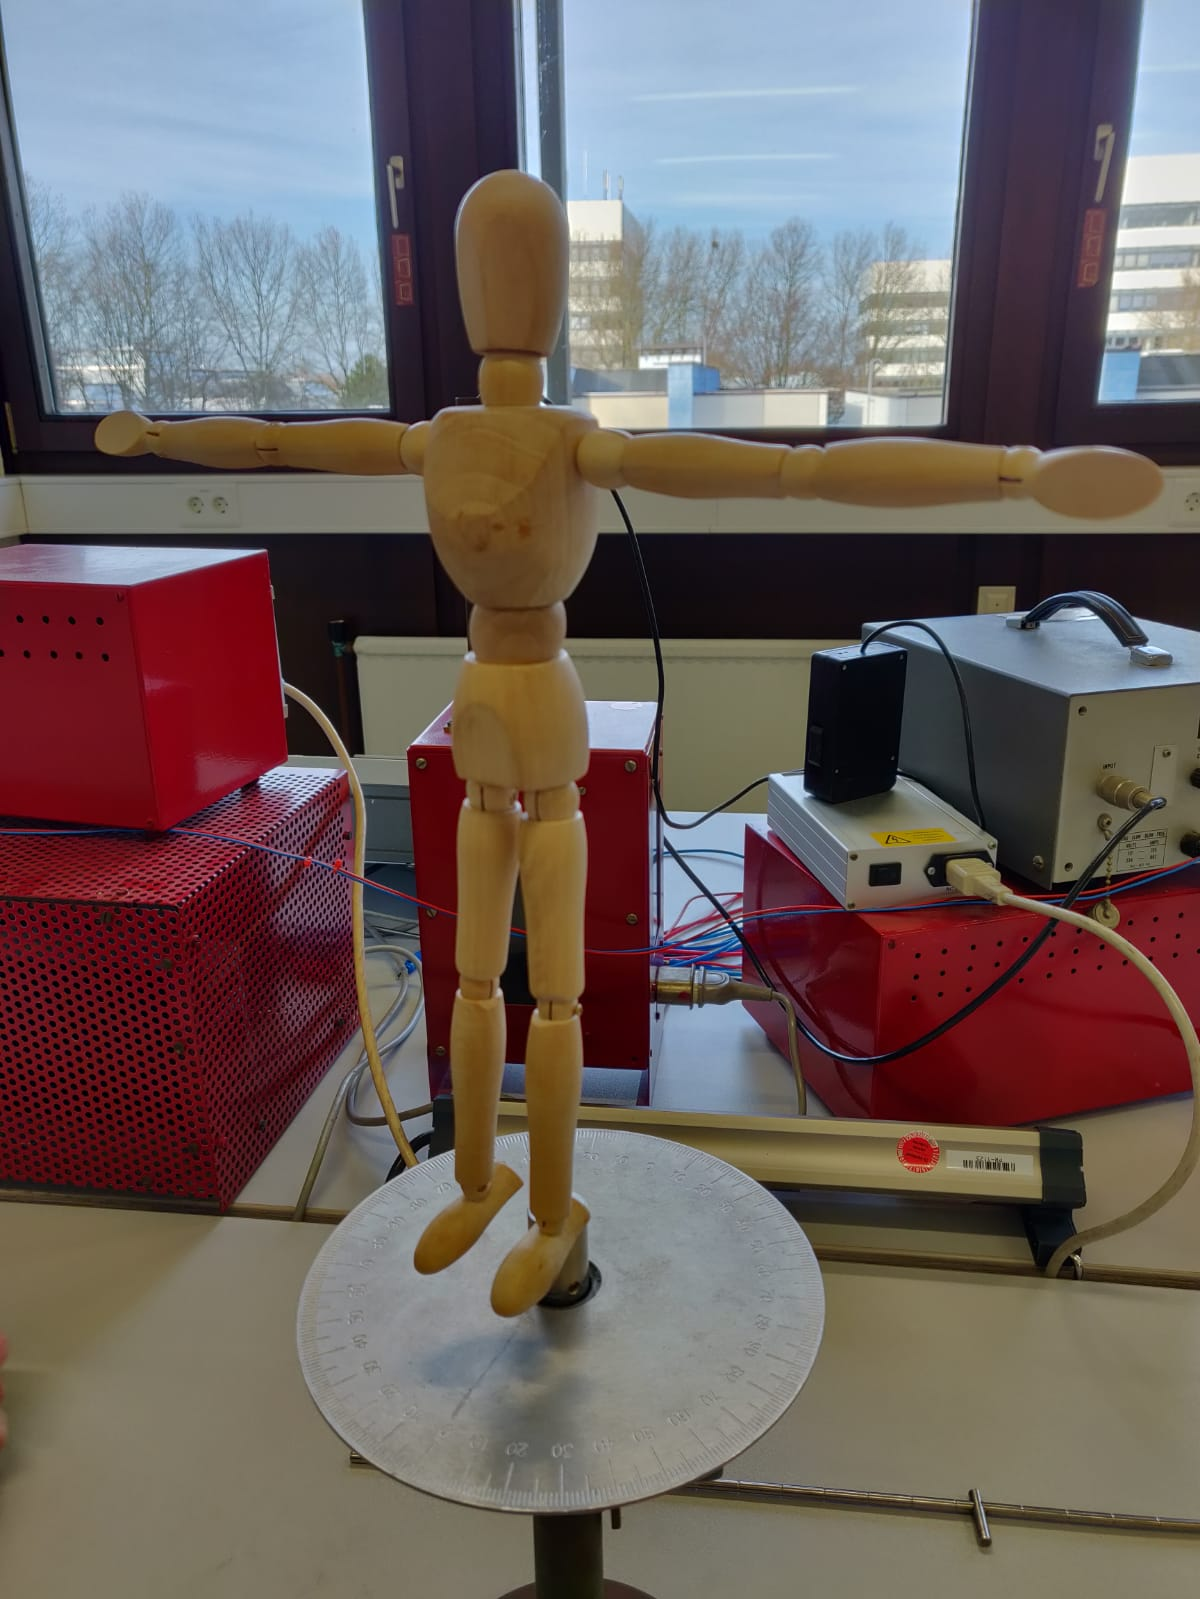
\includegraphics[scale=0.1]{content/data/PuppeTPose2.png}
    \caption{Versuchsaufbau mit einer sitzenden Puppe.}
    \label{fig:puppetpose}
\end{subfigure}
\caption{Die zwei Position von den Puppen.}
\label{fig:puppen}
\end{figure}
\FloatBarrier

